\documentclass[11pt,table,final,fleqn,xcolor={usenames,dvipsnames},unknownkeysallowed,handout]{beamer}
\usetheme[]{Frankfurt}
\usecolortheme{crane}

% \usepackage{listings}
% \usepackage{multimedia} % Movies
% \usepackage{fancyvrb,relsize}
% \usepackage{commath}
% \usepackage{graphicx}
% \usepackage{longtable}
% \usepackage[math]{iwona}
% \usepackage{wasysym}
% \usepackage{amsmath}
% \usepackage{amssymb}
% \usepackage[amssymb]{SIunits}
% \usepackage{tikz} % Drawing


\usepackage{listings}
\usepackage{multimedia} % Movies
\usepackage{fancyvrb,relsize}
\usepackage{commath}
\usepackage{graphicx}
\usepackage{array}
\usepackage{longtable}
\usepackage{algpseudocode} 
\usepackage{multirow}
\usepackage[math]{iwona}
\usepackage{wasysym}
% \usepackage[fleqn]{amsmath}
\usepackage{amssymb}
\usepackage{siunitx}
\usepackage{tikz} % Drawing
\usepackage{pgfplots}
\usepackage{pgfplotstable}
% \usepackage{fontspec}

% Presentation settings
\rowcolors[]{1}{maincolor!20}{maincolor!10}

\newcommand{\Fo}{\ensuremath{\mathit{Fo}}}

\lstset{language=Matlab,%
    %basicstyle=\color{red},
    basicstyle=\scriptsize\ttfamily,
    breaklines=true,%
    morekeywords={matlab2tikz},
    keywordstyle=\color{blue},%
    morekeywords=[2]{1}, keywordstyle=[2]{\color{black}},
    identifierstyle=\color{black},%
    stringstyle=\color{mylilas},
    commentstyle=\color{mygreen},%
    showstringspaces=false,%without this there will be a symbol in the places where there is a space
    numbers=none,%
%     numberstyle={\tiny \color{black}},% size of the numbers
%     numbersep=-2pt, % this defines how far the numbers are from the text
%     emph=[1]{for,end,break},emphstyle=[1]\color{red}, %some words to emphasise
emph=[2]{ones,int,str2double,long,single,simplify,diff,log,atan,solve,vpa,syms,doc,int,simplify,diff,log,atan,syms,interp3,interpn,histogram,ribbon,contourf,fzero,feval,fminsearch,fsolve,fminbnd,ezplot,varargin,optimset,odeset,ode15s,plotyy,ones,linprog,cftool,optimset,lsqnonlin}, emphstyle=[2]{\color{blue}},
    backgroundcolor=\color{gray!15},frame=tlbr, framerule=0pt,
    escapeinside={(*@}{@*)}
}

% To have the navigation circles without declaring subsections
\usepackage{remreset}% tiny package containing just the \@removefromreset command
\makeatletter
\@removefromreset{subsection}{section}
\makeatother
\setcounter{subsection}{1}

% For convenient figure inclusion
\DeclareGraphicsExtensions{.pdf,.png,.jpg}
\graphicspath{ {../img/} }


% \setmainfont{Yanone Kaffeesatz}
% \setmathfont(Digits,Latin,Greek)[Numbers={Lining,Proportional}]{Gentium Plus}

% TU/e colors
\definecolor{tuered}{RGB}{247,49,49}
\definecolor{tuefuchsia}{RGB}{214,0,74}
\definecolor{tuelila}{RGB}{214,0,123}
\definecolor{tuepurple}{RGB}{173,32,173}
\definecolor{tuedblue}{RGB}{16,16,115}
\definecolor{tueblue}{RGB}{0,102,204}
\definecolor{tuelblue}{RGB}{0,162,222}
\definecolor{tueorange}{RGB}{255,154,0}
\definecolor{tueyellow}{RGB}{255,221,0}
\definecolor{tuedyellow}{RGB}{206,223,0}
\definecolor{tuegreen}{RGB}{132,210,0}
\definecolor{tuedgreen}{RGB}{0,172,130}
\definecolor{tueblue2}{RGB}{0,146,181}

% For Matlab script colors
\definecolor{mygreen}{RGB}{28,172,0} % color values Red, Green, Blue
\definecolor{mylilas}{RGB}{170,55,241}

\makeatletter
% \definecolor{beamer@blendedblue}{rgb}{0.5,0.5,0.3} % changed this
\useoutertheme{smoothbars}
\useinnertheme{circles}

%%%%%%%%%%%%%%%%%%%%%%%%%%%%%%%%%%%%%%%%%%%%%%%%%%%%%%%%%%%%%%%%%%%%%%%%%%%
\definecolor{maincolor}{named}{tuelblue}
\definecolor{textcolorfg}{named}{white}
\definecolor{tuealert}{named}{tueblue}
%%%%%%%%%%%%%%%%%%%%%%%%%%%%%%%%%%%%%%%%%%%%%%%%%%%%%%%%%%%%%%%%%%%%%%%%%%%

\setbeamercolor{normal text}{fg=black,bg=white}
\setbeamercolor{alerted text}{fg=tuealert}
\setbeamercolor{example text}{fg=tuegreen!50!black}

\setbeamercolor{background canvas}{parent=normal text,bg=white}
\setbeamercolor{background}{parent=background canvas}

\setbeamercolor{title}{bg=maincolor,fg=textcolorfg} % Presentation title colors
\setbeamercolor{structure}{fg=maincolor,bg=textcolorfg}
\setbeamercolor{section in head/foot}{fg=textcolorfg,bg=maincolor}
\setbeamercolor{palette primary}{fg=textcolorfg,bg=maincolor} % changed this

\setbeamercolor{palette primary}{fg=maincolor,bg=textcolorfg} % changed this
\setbeamercolor{palette secondary}{use=structure,fg=structure.fg!100!tueblue} % changed this
\setbeamercolor{palette tertiary}{use=structure,fg=structure.fg!100!tuered} % changed this

\setbeamertemplate{navigation symbols}{} % ( Dont use )
\setbeamercolor{navigation symbols}{use=structure,fg=structure.fg!40!bg}
\setbeamercolor{navigation symbols dimmed}{use=structure,fg=structure.fg!20!bg}

\setbeamercolor{block title}{fg=textcolorfg,bg=maincolor}
\setbeamercolor{block body}{fg=black,bg=maincolor!10}

\def\colorize<#1>{%
  \temporal<#1>{\color{tuedblue!40!gray!40}}{\color{tuealert}}{\color{black}}}
  
\setlength{\mathindent}{0pt}

\makeatother

% Colored urls
\hypersetup{colorlinks,linkcolor=,urlcolor=tueblue}

% Vector format
\renewcommand{\vec}[1]{\mathbf{#1}}

\usetikzlibrary{decorations} % Drawing
\usetikzlibrary{patterns}
\usetikzlibrary{positioning}
\usetikzlibrary{shadows}
\usetikzlibrary{calc}
\usetikzlibrary{arrows}
\usetikzlibrary{decorations}
\usetikzlibrary{plotmarks}
\usetikzlibrary{shapes}
\usetikzlibrary{shadings}
\usetikzlibrary{intersections}
% Blocks
\tikzset{block/.style={rectangle,draw=maincolor,fill=maincolor!20,text width=10em,text centered,rounded corners,minimum height=4em,thick}}
\tikzset{emphblock/.style={rectangle,draw=maincolor,text centered,rounded corners,thick,top color=maincolor!10,bottom color=maincolor!30}}
% Dots
\tikzset{dot/.style={draw=tuered,circle,thick,minimum size=1mm,inner sep=0pt,outer sep=0pt,fill=white}}
\tikzset{fdot/.style={circle,draw=black,fill=black,,inner sep=1.5pt}}
\tikzset{gdot/.style={circle,draw=black,inner sep=3pt}}
\tikzset{cross/.style={cross out, draw=black, fill=none, minimum size=2*(#1-\pgflinewidth), inner sep=0pt, outer sep=0pt}, cross/.default={4pt}}
% Graphs and lines
\tikzset{line/.style={black,>=stealth',semithick}}
\tikzset{graph/.style={smooth,samples=400,tuered,semithick}}
\tikzset{interp/.style={dot,draw=tuealert,inner sep=1.5pt,minimum size=4pt,color=tuealert,fill=none}}
\tikzset{intblock/.style={line,draw=tuefuchsia,fill=tuefuchsia!50!white,fill opacity=0.3,opacity=0.6}}
\tikzset{intdot/.style={line,dot,draw=tuefuchsia,fill=tuefuchsia,opacity=0.6}}
\tikzset{gridline/.style={lightgray,ultra thin,dashed}}


\newcolumntype{L}[1]{>{\raggedright\arraybackslash}p{#1}}
\newcolumntype{R}[1]{>{\raggedleft\arraybackslash}p{#1}}

% \pgfplotsset{
% % every axis y label/.append style={at={axis cs:14,14},rotate=0,anchor=south east}
% exery axis/.style={ylabel near ticks},
% }


\renewcommand*\familydefault{\sfdefault}  % Use sans font
% 
% \usepackage{pgfpages}
% \pgfpagesuselayout{4 on 1}[border shrink=5mm]

% PRESENTATION SPECIFICS
\title{Matlab and Programming 1}
\subtitle{Programming basics and algorithms}

\author[I.~Roghair]{\underline{Ivo~Roghair}, Martin van Sint Annaland}

\institute{Chemical Process Intensification\\Eindhoven University of Technology}

\date

% BEGIN PRESENTATION
\begin{document}
\lstset{language=Matlab,%
    %basicstyle=\color{red},
    basicstyle=\footnotesize\ttfamily,
    breaklines=true,%
    morekeywords={matlab2tikz},
    keywordstyle=\color{blue},%
    morekeywords=[2]{1}, keywordstyle=[2]{\color{black}},
    identifierstyle=\color{black},%
    stringstyle=\color{mylilas},
    commentstyle=\color{mygreen},%
    showstringspaces=false,%without this there will be a symbol in the places where there is a space
    numbers=none,%
%     numberstyle={\tiny \color{black}},% size of the numbers
%     numbersep=-2pt, % this defines how far the numbers are from the text
%     emph=[1]{for,end,break},emphstyle=[1]\color{red}, %some words to emphasise
    emph=[2]{ones,int,simplify,diff,log,atan,syms,doc,int,simplify,diff,log,atan,syms,interp3,interpn,histogram,ribbon,contourf,fzero,feval,fminsearch,fsolve,fminbnd,ezplot,varargin,optimset,odeset,plotyy,ones,linprog,cftool,optimset,lsqnonlin}, emphstyle=[2]{\color{blue}},
    backgroundcolor=\color{gray!15},frame=tlbr, framerule=0pt,
    escapeinside={(*@}{@*)}
}

\frame[plain]{
  \titlepage
}

\section{Introduction}
\subsection*{Introduction}
\begin{frame}[label=contents]
  \frametitle{Today's outline}
  \mode<beamer>{
    \only<1>{\tableofcontents}
  }
  \only<2>{\tableofcontents[currentsection]}
\end{frame}

\begin{frame}[t]
 \frametitle{Programming}
 \vskip1em
   \tikzstyle{every picture}-=[remember picture]
  {\LARGE \vspace{-1em}``Everybody in this country should learn to program a computer, because it teaches you to think..''\\
   {\vspace{1em}\hspace{10em} ---Steve Jobs}}
   \begin{tikzpicture}[remember picture,overlay]{
    \node[xshift=-0.2cm,yshift=-0.2cm, anchor=south west] at (current page.south west) {
\includegraphics[width=0.4\textwidth]{img/jobs.png}};}
   \end{tikzpicture}
\end{frame}

\begin{frame}
 \frametitle{Why?}
 \begin{itemize}[<+->]
  \item Scientific techniques depend in an increasing fashion upon computer programs and simulation methods
  \item Knowledge of programming allows you to automate routine tasks 
  \item Ability to understand algorithms by inspection of the code 
  \item Learn to think by dissecting a problem into smaller bits 
 \end{itemize}\vskip2em
 \begin{columns}
  \column<1->{0.23\textwidth}
  \tikz\node[circle,draw,very thick,maincolor,
           text=white,minimum size=\columnwidth,
           path picture={
               \node at (path picture bounding box.center){
                   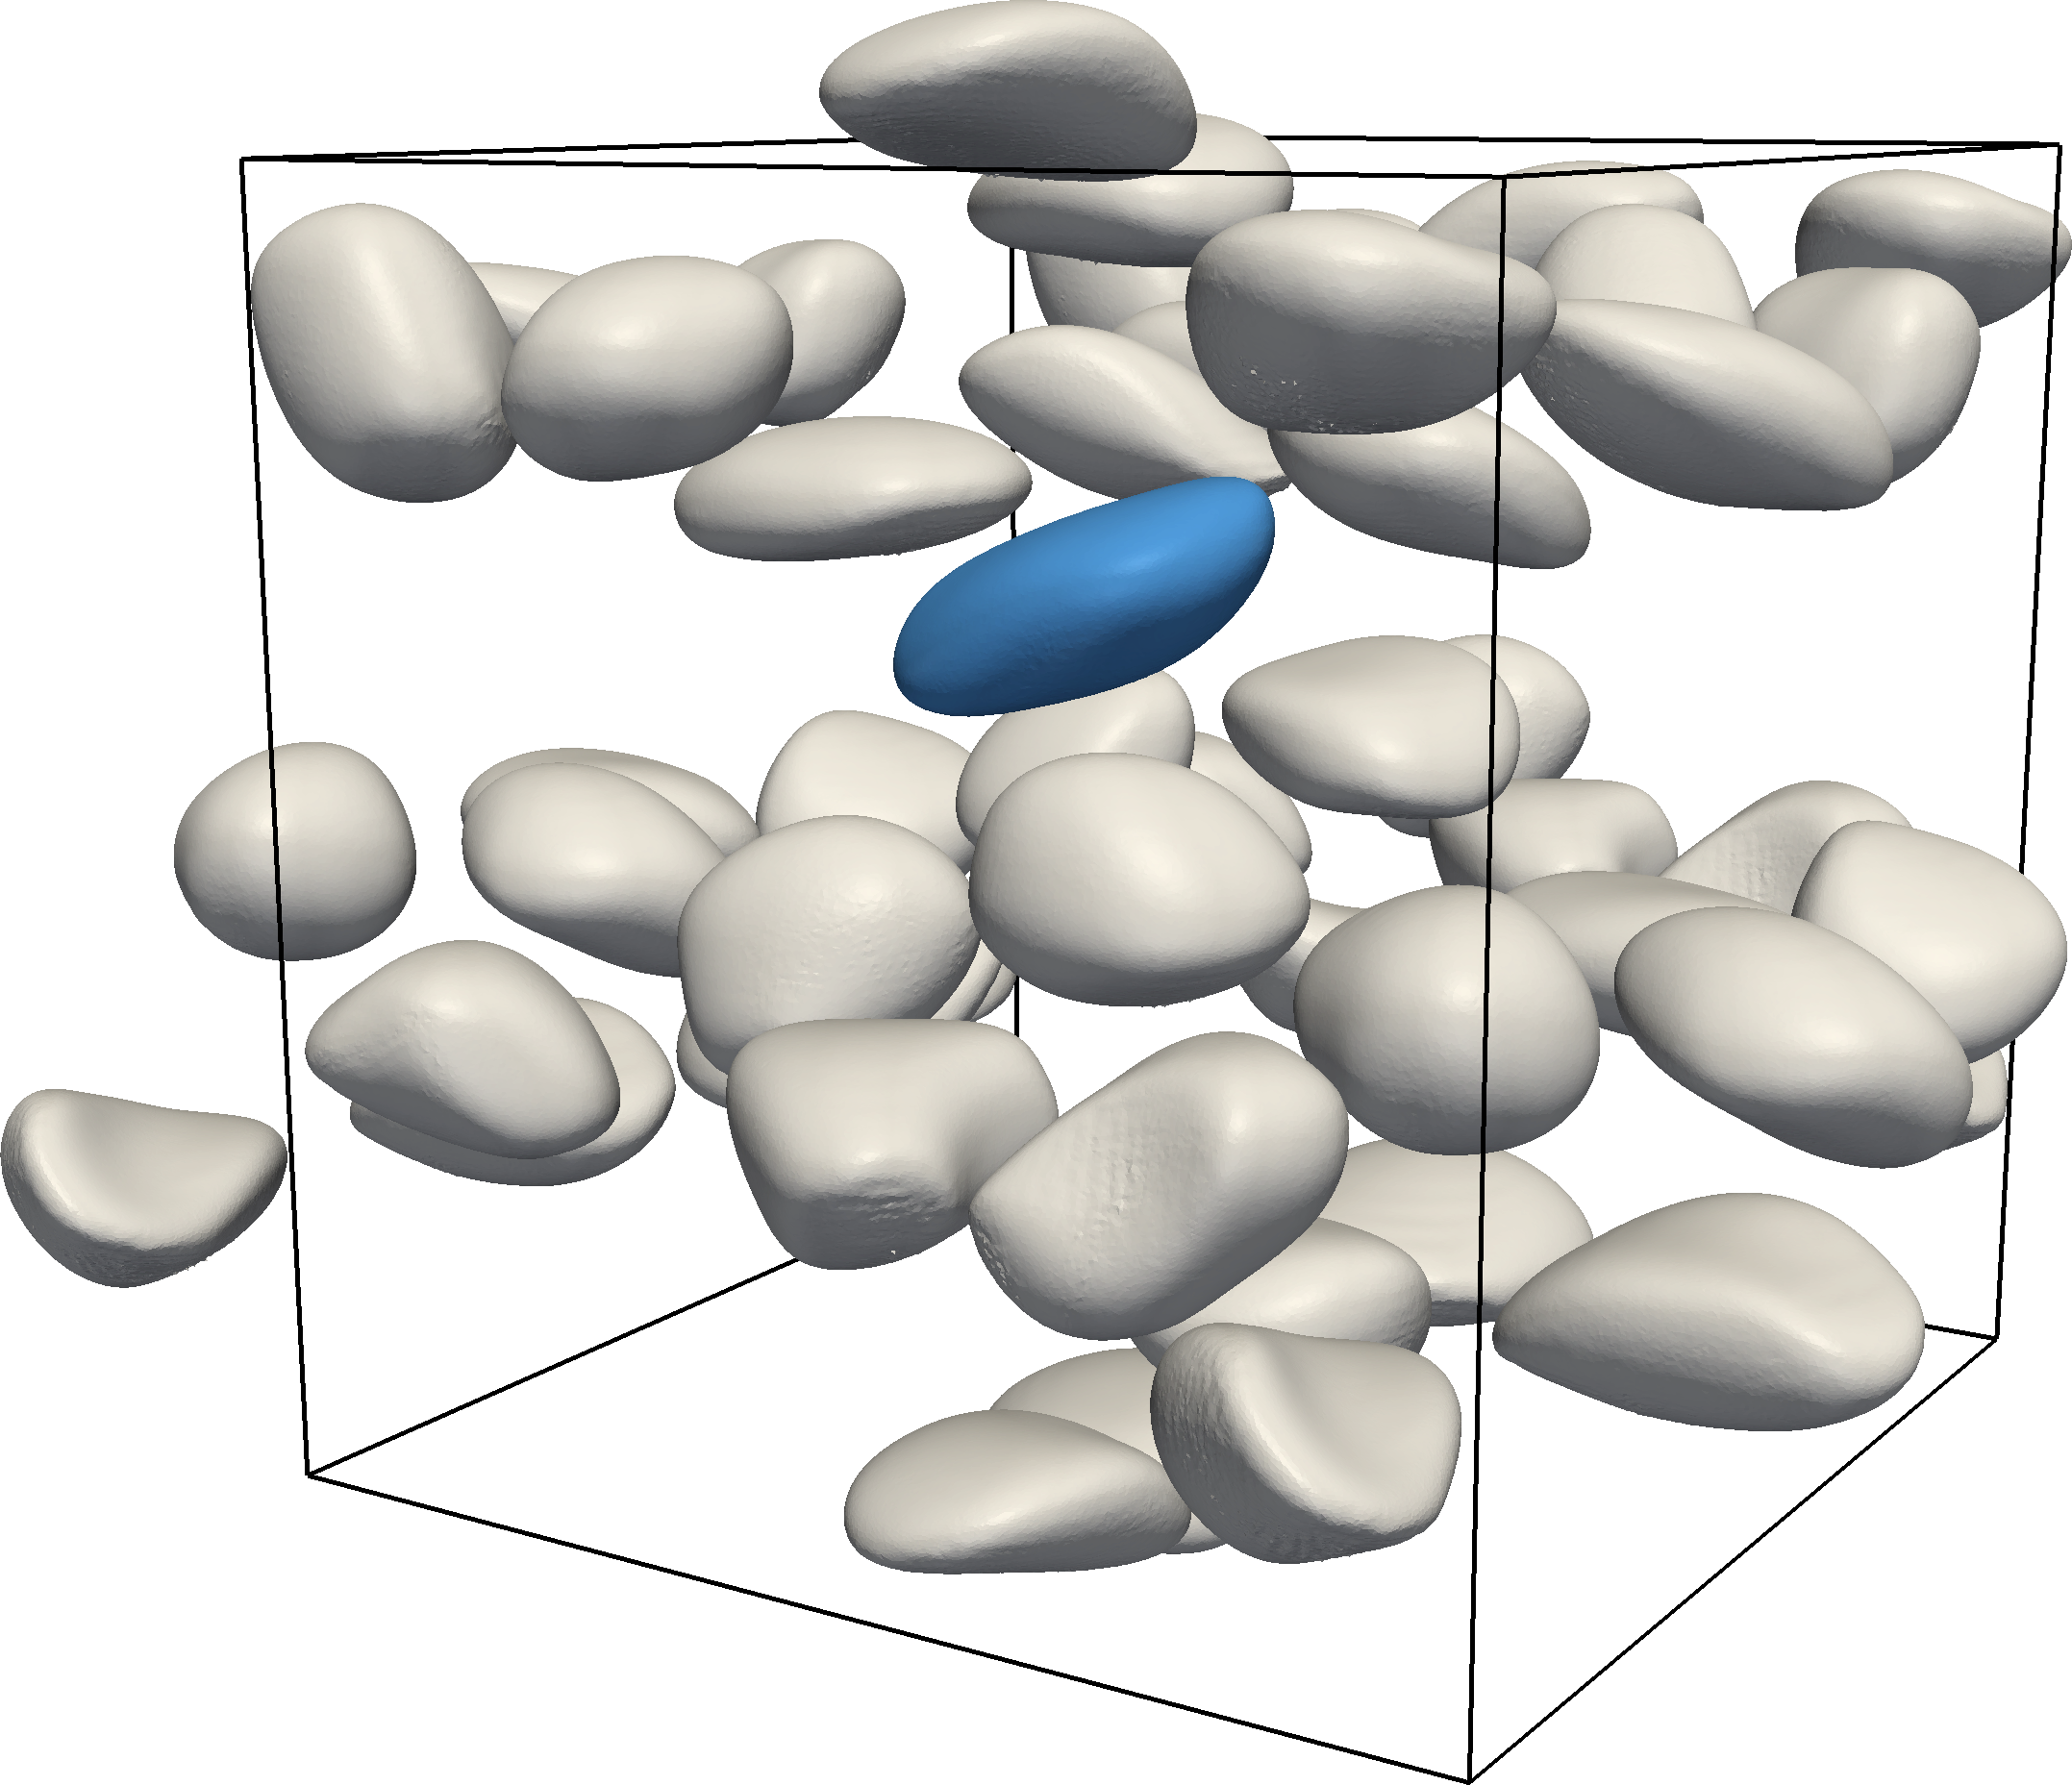
\includegraphics[width=\columnwidth]{img/sim1.png}
               };
           }]{};
  \column<2->{0.23\textwidth}
  \tikz\node[circle,draw,very thick,maincolor,
           text=white,minimum size=\columnwidth,
           path picture={
               \node at (path picture bounding box.center){
                   
\includegraphics[width=1.1\columnwidth]{img/automate.jpg}
               };
           }]{};
  \column<3->{0.23\textwidth}
  \tikz\node[circle,draw,very thick,maincolor,
           text=white,minimum size=\columnwidth,
           path picture={
               \node at (path picture bounding box.center){
                   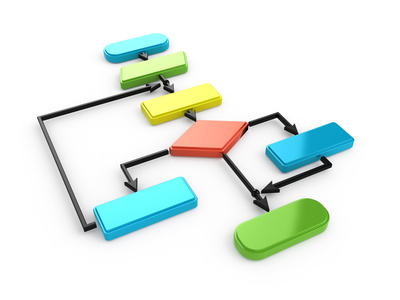
\includegraphics[width=1.2\columnwidth]{img/algorithm.jpg}
               };
           }]{};
  \column<4>{0.23\textwidth}
  \tikz\node[circle,draw,very thick,maincolor,
           text=white,minimum size=\columnwidth,
           path picture={
               \node at (path picture bounding box.center){
                   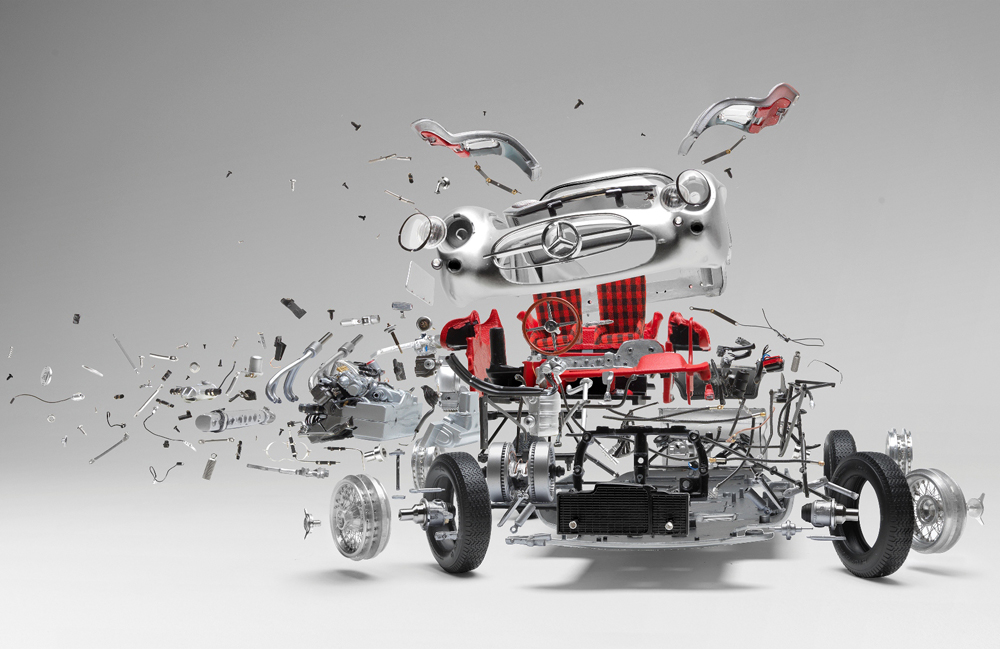
\includegraphics[width=1.5\columnwidth]{img/dissect.jpg}
               };
           }]{};
 \end{columns}
\end{frame}

\begin{frame}[fragile]
 \frametitle{Getting started}
  Start Matlab, and enter the following commands on the command line. Evaluate the output.
  \pause
  \begin{lstlisting}
>> 2 + 3        % Some simple calculations
>> 2*3
>> 2*3^2        % Powers are done with ^ (*@ \pause @*)
>> a = 2        % Storing values into the workspace
>> b = 3
>> c = (2*3)^2  % Parentheses set priority
>> 8/a-b (*@ \pause @*)
>> sin(a)       % Mathematical functions can be used 
>> sin(0.5*pi)  % pi is an internal Matlab variable
>> 1/0          % Infinity is a thing ...
>> sqrt(-1)     % ... as are imaginary numbers
  \end{lstlisting}
\end{frame}

\begin{frame}
 \frametitle{Introduction to programming}
 \begin{block}{What is a program?}
  \emph{A program is a sequence of instructions that is written to perform a certain task on a computer.} % SOURCE http://www.greenteapress.com/thinkpython/html/thinkpython002.html
  \end{block}
  \begin{itemize}
    \item The computation might be something mathematical, such as solving a system of equations or finding the roots of a polynomial
    \item It can also be a symbolic computation, such as searching and replacing text in a document 
    \item A program may even be used to compile another program
    \item A program consists of one or more \emph{algorithms}
  \end{itemize}
\end{frame}

\begin{frame}
 \frametitle{Getting started}
 \begin{itemize}
   \item Use an \emph{integrated development environment}
   \begin{itemize}
     \item Matlab
     \item MS Visual Studio/Code
     \item Eclipse
     \item Dev C++
     \item IDLE, Canopy (express)
   \end{itemize}
   \item Create a simple program:
   \begin{itemize}
     \item Hello world
     \item Find the roots of a parabola
     \item Find the greatest common divisor of two numbers
   \end{itemize}
 \end{itemize}
\end{frame}

\begin{frame}
 \frametitle{Some often used programming languages}
 \fontsize{7.2pt}{7.2}\selectfont
 \begin{columns}[T]
   \column{0.45\textwidth}
   \begin{block}<1->{Python}
     \begin{itemize}
       \item Many functionalities available
       \item Smooth learning curve
       \item Slow compared to compiled languages
       \item Many freely available editors
     \end{itemize}
   \end{block}
    \begin{block}<2->{Pascal}
     \begin{itemize}
       \item Limited number of libraries available
       \item Steep learning curve
       \item Compiled language, may be fast
       \item Some free compilers (fpc)
     \end{itemize}
   \end{block}
   \column{0.45\textwidth}
   \begin{block}<3->{C / C++ / C\#}
     \begin{itemize}
       \item Many functionalities available 
       \item Steeper learning curve
       \item Needs compilation, very fast (HPC)
       \item Freely available (gcc, MSVC)
     \end{itemize}
   \end{block}
   \begin{block}<4->{Spreadsheet (Excel, Google Docs, ...)}
     \begin{itemize}
       \item High availability
       \item Low learning curve
       \item Very limited for larger problems, unbeatable for quick calculations
       \item Not always free
     \end{itemize}
   \end{block}
 \end{columns}
    \begin{block}<5>{Matlab}
     \begin{columns}[T]
     \column{0.5\textwidth}
     \begin{itemize}
       \item Many functionalities built-in (80+ toolkits!)
       \item Slow compared to compiled languages
       \end{itemize}
       \column{0.5\textwidth}
       \begin{itemize}
       \item Fairly smooth learning curve
       \item Needs a license (alternatives: SciLab, GNU Octave)
     \end{itemize}
     \end{columns}
   \end{block}
\end{frame}

\begin{frame}
\frametitle{Versatility of Matlab}
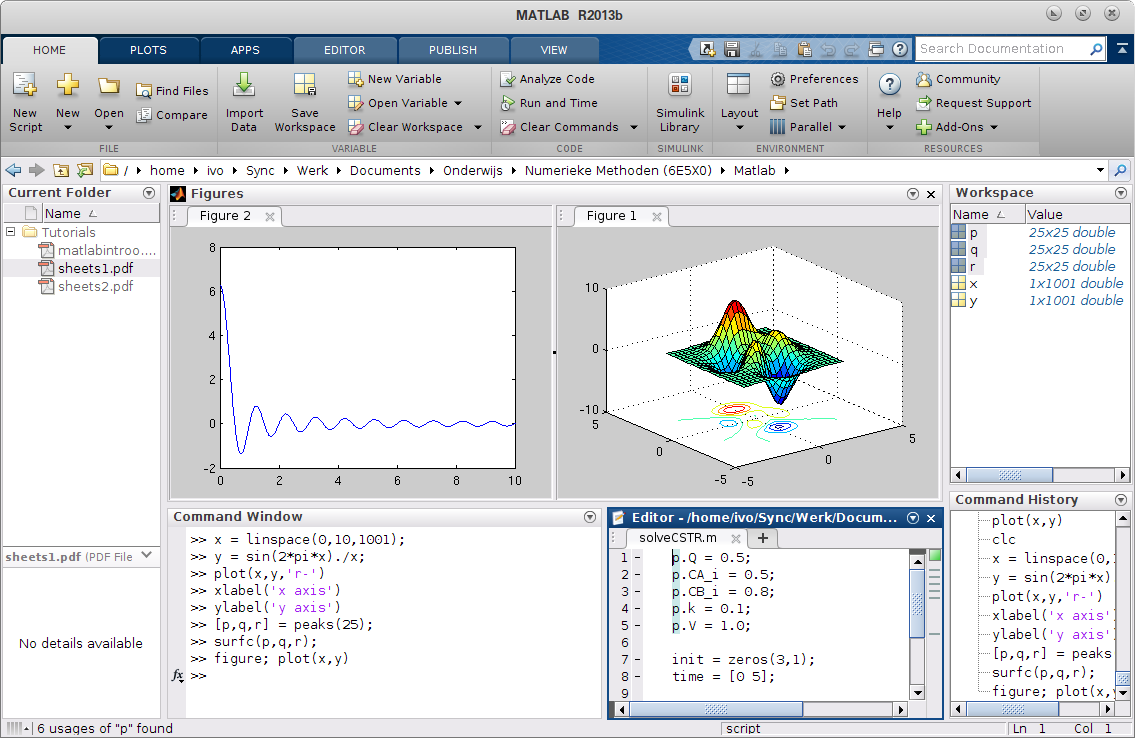
\includegraphics[width=\textwidth]{matlab.png}
\end{frame}

\begin{frame}
\frametitle{Versatility of Matlab: ODE solver}
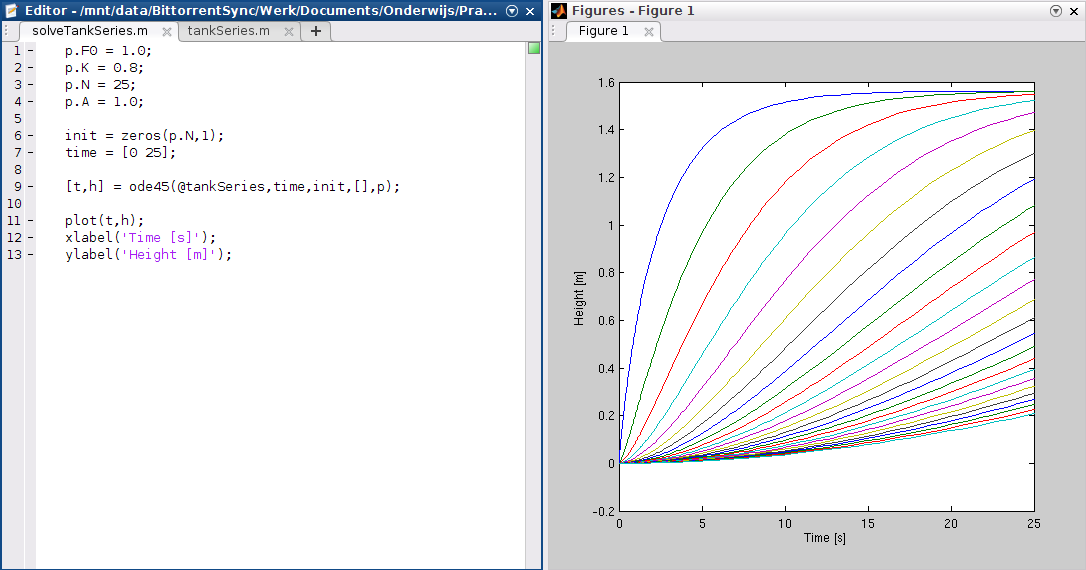
\includegraphics[width=\textwidth]{odesol.png}
\end{frame}

\begin{frame}[fragile]
\frametitle{Versatility of Matlab: Image analysis}
\begin{columns}
  \column{0.5\textwidth}
\begin{lstlisting}
I = imread('bubbles.png');
BW = rgb2gray(I);
E = edge(BW, 'canny');
F = imfill(E, 'holes');
result = regionprops(F);
\end{lstlisting}  
\column{0.5\textwidth}
  \vfill
  \includegraphics<1>[width=\columnwidth]{bub1.png}
  \includegraphics<2>[width=\columnwidth]{bub2.png}
  \includegraphics<3>[width=\columnwidth]{bub3.png}
  \includegraphics<4>[width=\columnwidth]{bub4.png}
\end{columns}
\end{frame}

\begin{frame}
\frametitle{Versatility of Matlab: Curve fitting}
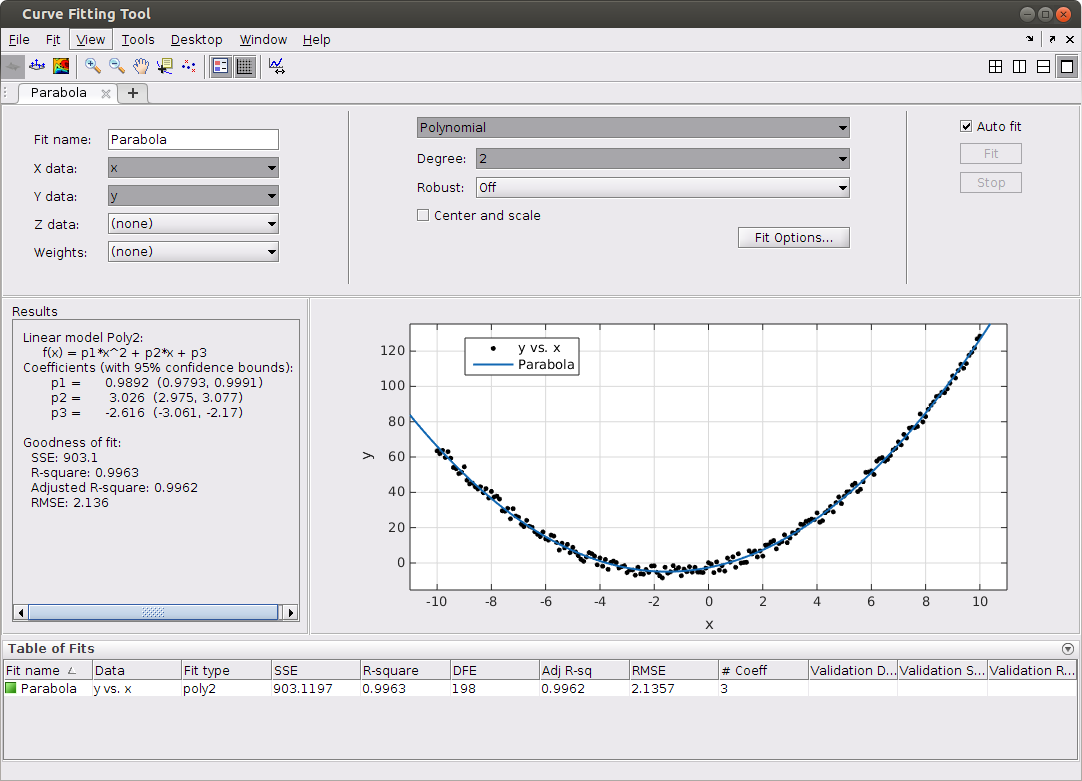
\includegraphics[width=\textwidth]{cftool.png}
\end{frame}

\begin{frame}
\frametitle{Matlab help}
\begin{itemize}[<+->]
  \item Matlab documentation: \lstinline$doc$ or \lstinline$help$ function
  \item Canvas page
  \item Introduction to Numerical Methods and Matlab Programming for Engineers. T. Young and M.J. Mohlenkamp (2015). GNU-licensed document, online
%   \item Interactive Matlab Course. Pieter van Zutven (2010). See also \url{http://www.imc.tue.nl/}
  \item Search the web!
\end{itemize}
\vspace{-2em}
\flushright\tikz{\node[] at (4cm,-2cm) {
\includegraphics[width=0.5\textwidth]{img/help.jpg}};}
\end{frame}
%
\section{Variables}
\subsection*{Introduction}
\againframe<2>{contents}
\begin{frame}
 \frametitle{Terminology}
 \begin{description}
  \item[Variable] Piece of data stored in the computer memory, to be referenced and/or manipulated
  \item[Function] Piece of code that performs a certain operation/sequence of operations on given input
  \item[Operators] Mathematical operators (e.g. \lstinline$ + - *$ or \lstinline$/$), relational (e.g. \lstinline$< >$or \lstinline$==$, and logical operators (\lstinline$&&$, \lstinline$||$)
  \item[Script] Piece of code that performs a certain sequence of operations without specified input/output
  \item[Expression] A command that combines variables, functions, operators and/or values to produce a result.
 \end{description}
\end{frame}

\subsection*{Vectors}
\begin{frame}[fragile]
 \frametitle{Variables in Matlab}
  \begin{itemize}
   \item Matlab stores variables in the \emph{workspace}\pause
   \item You should recognize the difference between the \emph{identifier} of a variable (its name, e.g. \lstinline$x$, \lstinline$setpoint_p$), and the data that it actually stores (e.g. 0.5)\pause
   \item Matlab also defines a number of variables by default, e.g. \lstinline$eps$, \lstinline$pi$ or \lstinline$i$.\pause
   \item You can assign a variable by the \lstinline$=$ sign:
   \begin{lstlisting}
>> x = 4*3
x =
    12
   \end{lstlisting}\pause
   \item If you don't assign a variable, it will be stored in \lstinline$ans$
   \item Clearing the workspace is done with \lstinline$clear$.
 \end{itemize}
\end{frame}

\begin{frame}[fragile]
  \frametitle{Vectors in Matlab (1)}
  A row vector:
  \begin{lstlisting}
>> v = [0 1 2 3]
  \end{lstlisting}\pause
  A column vector by separating elements with semi-colons:
  \begin{lstlisting}
>> u = [9; 10; 11; 12; 13; 14; 15]
  \end{lstlisting}\pause
  Access (i.e. read) an entry in a vector:
  \begin{lstlisting}
>> u(2)
  \end{lstlisting}\pause
  Manipulate the value of that entry:
  \begin{lstlisting}
>> u(2)=47
  \end{lstlisting}\pause
  Get a slice of a vector:
  \begin{lstlisting}
>> u([2 3 4]) % With colon operator: u(2:4)
  \end{lstlisting}\pause
  Transposing vectors:
  \begin{lstlisting}
>> w = v'
  \end{lstlisting}
\end{frame}

\begin{frame}[fragile]
  \frametitle{Vectors in Matlab (2)}
  Manual definition may be cumbersome. A colon (\lstinline$:$) generates a list:
  \begin{lstlisting}
>> a = 1:10      % Default stride is 1
>> x = -1:.1:1   % start:stride:stop specifies list
  \end{lstlisting}\pause
  Or, when you prefer to set the \emph{number of elements} instead of the step size:
  \begin{lstlisting}
>> y = linspace(0,10,11)
>> p = logspace(2,6,5)
  \end{lstlisting}\pause
  Manipulating multiple components:
  \begin{lstlisting}
>> y([1 4:7]) = 1
  \end{lstlisting}\pause
  Or (by supplying a vector instead of a scalar):
  \begin{lstlisting}
>> y([1 4:7]) = 16:20 % equivalent to y([1 4 5 6 7]) = [16 17 18 19 20]
  \end{lstlisting}
\end{frame}

\begin{frame}[fragile]
 \frametitle{Practice}
 Given a vector 
 \[ 
    x = \left[2 \ 4 \ 6 \ 8 \ 10 \ 12 \ 14 \ 16 \ 18 \ 20 \ 30 \ 40 \ 50 \ 60 \ 70 \ 80 \right]
 \]
 \begin{itemize}
  \item Find a way to define the vector without typing all individual elements\pause
  \item Investigate the meaning of the following commands:
  \begin{lstlisting}
>> y = x(5:end)
>> y(4)
>> y(4) = []
>> sum(x)
>> mean(x)
>> std(x)
>> max(x)
>> fliplr(x)
>> diff(x)
  \end{lstlisting}
 \end{itemize}
\end{frame}

\begin{frame}[fragile]
  \frametitle{Operations on vectors (1)}
  \begin{lstlisting}
>> e = 1:5
>> f = 2*e
>> g = 4*f + 20 (*@ \pause @*)
>> h = e^2
  \end{lstlisting}\pause
  ... wait ... what's that?
  \begin{lstlisting}[basicstyle=\color{red}\footnotesize\ttfamily,keywordstyle={\color{red}}, identifierstyle=\color{red}]
Error using  ^ 
Inputs must be a scalar and a square matrix.
To compute elementwise POWER, use POWER (.^) instead.
  \end{lstlisting}\pause
  Matlab uses matrix operations by default, we should use a dot operator to make operations element-wise for \lstinline$*$, \lstinline$/$ and \lstinline$^$.
  \begin{lstlisting}
>> e.^2
  \end{lstlisting}
\end{frame}

\begin{frame}[fragile]
  \frametitle{Operations on vectors (2)}
   To demonstrate the matrix product:
  \begin{lstlisting}
>> p = [1; 1; 1]
>> q = [1 2 3]
>> p*q   % which is not equal to q*p
  \end{lstlisting}\pause
  All kinds of mathematical functions on vectors typically operate on elements:
  \begin{lstlisting}
>> x = linspace(0,2*pi,100);
>> s = sin(x)
>> e = exp(x)
  \end{lstlisting}
\end{frame}

\begin{frame}
 \frametitle{Building blocks: Mathematics and number manipulation}
 Programming languages usually support the use of various mathematical functions (sometimes via a specialized library). Some examples of the most elementary functions in Matlab:
    \begin{longtable}{l!{\vrule}l}
      Command        & Explanation \\ \hline
      \texttt{cos(x), sin(x), tan(x)} & Cosine, sine or tangens of $x$ \\
      \texttt{mean(x), std(x)} & Mean, st. deviation of vector $x$ \\
      \texttt{exp(x)} & Value of the exponential function $e^x$ \\
      \texttt{log10(x), log(x)} & Base-10/Natural logarithm of $x$ \\
      \texttt{floor(x)} & Largest integer smaller than $x$ \\
      \texttt{ceil(x)} & Smallest integer that exceeds $x$ \\
      \texttt{abs(x)} & Absolute value of $x$ \\
      \texttt{size(x)} & Size of a vector $x$ \\
      \texttt{length(x)} & Number of elements in a vector $x$ \\
      \texttt{rem(x,y)} & Remainder of division of $x$ by $y$\\
    \end{longtable}
\end{frame}

\begin{frame}[fragile]
  \frametitle{Printing results}
  You can prevent displaying the outcome of a command by adding a semi-colon at the end of a line:
  \begin{lstlisting}
>> c = linspace(0,10,11);
>> length(c)
>> c
>> size(c)
  \end{lstlisting}\pause
  Altering the display format can be done using the \lstinline$format$ command:
  \begin{lstlisting}
>> format compact % loose
>> format long    % short
  \end{lstlisting}
\end{frame}

\subsection*{Simple plotting}
\begin{frame}[fragile]
  \frametitle{Simple plotting}
  Make a plot of the following table
   \begin{longtable}{l!{\vrule}ccccc}
%    \rowcolors[]{1}{maincolor!20}{maincolor!10}
      T ($^\circ$C) & 5   &  20  & 30   & 50   & 55 \\
      $\mu$ (Pa$\cdot$s)  & 0.08& 0.015& 0.009& 0.006& 0.0055 \\
    \end{longtable} \pause
  \begin{lstlisting}
>> x = [ 5 20 30 50 55 ]
>> y = [ 0.08 0.015 0.009 0.006 0.0055]
\end{lstlisting}
\begin{onlyenv}<1-2>
  \begin{lstlisting}
>> plot(x,y)
  \end{lstlisting}
\end{onlyenv}
\begin{onlyenv}<3>
  \begin{lstlisting}
>> plot(x,y,'*')
  \end{lstlisting}
\end{onlyenv}
\begin{onlyenv}<4>
  \begin{lstlisting}
>> plot(x,y,'r--')
  \end{lstlisting}
\end{onlyenv}
\begin{onlyenv}<5>
  \begin{lstlisting}
>> plot(x,y,'ko-','LineWidth',2)
  \end{lstlisting}
\end{onlyenv}
\begin{lstlisting}
>> xlabel('Temperature [^\circC]')
>> ylabel('Viscosity [Pa s]')
>> title('Experiment 1')
  \end{lstlisting}
\end{frame}

\begin{frame}[fragile]
 \frametitle{Practice}
 Create plots of the following functions in a single figure for $x \in \left\{0,2\pi\right\}$:
  \[
    y_1 = \cos x 
  \]
  \[
    y_2 = \arctan x 
  \]
  \[
    y_3 = \frac{\sin x }{x}
  \]
  \pause
  Strategies to draw multiple graphs in 1 figure:
 \begin{lstlisting}
>> plot(x,y1,x,y2,x,y3)
 \end{lstlisting}
  \begin{lstlisting}
>> plot(x,y1)
>> hold on; % Maintain drawn plots in current figure
>> plot(x,y2)
>> plot(x,y3) % The 'hold-property' was already set
  \end{lstlisting}
\end{frame}

\subsection*{Matrices}
\begin{frame}[fragile]
  \frametitle{Matrices in Matlab}
  \begin{columns}[T]
   \column{0.35\textwidth}
    Matrix A is defined as:
    \[
    A = \begin{bmatrix}
      8 & 1 & 6 \\
      3 & 5 & 7 \\
      4 & 9 & 2
    \end{bmatrix}\]
    \pause
    \column{0.65\textwidth}
    In Matlab:
  \begin{lstlisting}
>> A = [ 8 1 6; 3 5 7; 4 9 2]
  \end{lstlisting}
  \end{columns}
  \pause
  Elements can be accessed/manipulated by the following syntax:
  \begin{lstlisting}
>> A(3,1) % Third row, first column, also A(3)
>> A(3,:) = [2 4 8] % Set entire third row
>> A(:,3) % Print third column
>> A(A>5) = 2 % Set elements by condition
  \end{lstlisting}\pause
  There are a few functions that help creating matrices:
  \begin{lstlisting}
>> A = zeros(4)  % A 4x4 matrix with zeros
>> A = ones(4,1) % A 4-element vector with ones
>> A = eye(3)    % Identity matrix of 3x3
>> A = rand(3,4) % A 3x4 matrix with random numbers
  \end{lstlisting}
\end{frame}

\begin{frame}[fragile]
 \frametitle{Practice}
 \begin{itemize}
  \item Find a \emph{short} Matlab expression to create the following matrix:
  \[
   A = \begin{bmatrix}
        1 & 2 & 3 & 4 & 5 & 6 & 7\\
        9 & 7 & 5 & 3 & 1 & -1 & -3 \\
        4 & 8 & 16 & 32 & 64 & 128 & 256 \\
       \end{bmatrix}
  \]\pause
  \item Investigate the command \lstinline$max(A)$. What does it give?
  \item How to obtain the maximum for each row?
  \item Use a vector multiplication to compute the following matrix:
    \[
   A = \begin{bmatrix}
	1 & 1 & 1 & 1 \\
        2 & 2 & 2 & 2 \\
        3 & 3 & 3 & 3 \\
        4 & 4 & 4 & 4 \\
       \end{bmatrix}
  \]
 \end{itemize}
\end{frame}

\begin{frame}[fragile]
 \frametitle{Datatypes and variables}
 Matlab uses different types of variables:
     \begin{longtable}{l!{\vrule}l}
      Datatype        & Example \\ \hline
      \texttt{string} & \lstinline$'Wednesday'$ \\
      \texttt{integer}& \lstinline$15$ \\
      \texttt{float}  & \lstinline$0.15$ \\
      \texttt{vector} & \lstinline$[0.0; 0.1; 0.2]$ \\
      \texttt{matrix} & \lstinline$[0.0 0.1 0.2; 0.3 0.4 0.5]$ \\
      \texttt{struct} & \lstinline$sct.name = 'MyDataName'$ \\
                      & \lstinline$sct.number = 13$ \\
      \texttt{logical}& \lstinline$0$ (false)  \\
                      & \lstinline$1$ (true) \\
    \end{longtable}
\end{frame}

\begin{frame}[fragile]
 \frametitle{About variables}
 \begin{itemize}
   \item Matlab variables can change their type as the program proceeds (this is not common for other programming languages!):
   \begin{lstlisting}
>> s = 'This is a string'
s =
This is a string
>> s = 10
s =
    10
\end{lstlisting}
    \item Vectors and matrices are essentially \emph{arrays} of another data type. A vector of \lstinline$struct$ is therefore possible.
    \item Variables are \emph{local} to a function (more on this later).
\end{itemize}
\end{frame}

\section{Creating algorithms}
\subsection*{Control statements}
\againframe<2>{contents}
\begin{frame}[fragile]
 \frametitle{Building blocks: conditional statements}
  \lstinline$if$-statement: Check whether a (set of) condition(s) is met. \\ 
  \vskip1em \pause
  \begin{lstlisting}
num = floor (10 * rand + 1);
guess = input ('Your guess please : ');
if ( guess ~= num )
  disp (['Wrong, it was ',num2str(num),'. Kbye.']);
else
    disp ('Correct !') ;
end
  \end{lstlisting}
  \pause
  \begin{columns}[T]
    \column{0.5\textwidth}
    Other relational operators
      \begin{longtable}{l!{\vrule}l}
      \hline
      \lstinline$==$& is equal to \\ 
      \lstinline$<=$& is less than or equal to\\
      \lstinline$>=$&is  greater than or equal to\\
      \lstinline$<$& is less than \\
      \lstinline$>$& is greater than \\
      \hline
    \end{longtable}  
    \column{0.5\textwidth}
      Combining conditional statements
      \begin{longtable}{l!{\vrule}l}
      \hline
      \lstinline$&&$& and \\ 
      \lstinline$||$& or\\
      \lstinline$xor$& exclusive or\\
      \hline
    \end{longtable}  
  \end{columns}
\end{frame}

\begin{frame}[fragile]
 \frametitle{Building blocks: loops}
  \lstinline$for$-loop: Performs a block of code a certain number of times. \\ 
  \vskip1em \pause
  \begin{lstlisting}
>> p(1) = 1;
>> p(2) = 1;
>> for i = 2:10
p(i+1) = p(i)+p(i-1);
end
>> p
p =
   1   1   2   3   5   8  13  21  34  55  89
  \end{lstlisting}
\end{frame}

\begin{frame}[fragile]
 \frametitle{Building blocks: indeterminate repetition}
  \lstinline$while$-loop: Performs and repeats a block of code until a certain condition. \\ 
  \vskip1em \pause
  \begin{lstlisting}
num = floor (10* rand +1) ;
guess = input ('Your guess please : ');

while ( guess ~= num )
    guess = input ('That is wrong. Try again ... ');
end

if (isempty(guess))
    disp('No number supplied - exit');
else
    disp ('Correct!');
end
  \end{lstlisting}
\end{frame}

%%%% Example
\begin{frame}[fragile]
 \frametitle{Example algorithm}
 Compute the factorial of $N$: $N! = N\cdot(N-1)\cdot(N-2)\cdots 2\cdot 1$\\ \vskip1em
 How to deal with this? \vfill
 \begin{columns}[T]
   \column{0.3\textwidth}
   \begin{block}<2->{Naive approach}
       \begin{lstlisting}
Z = 1;
Z = Z*2;
Z = Z*3;
Z = Z*4;
... etc ...      
       \end{lstlisting}
   \end{block}
   \column{0.3\textwidth}
   \begin{block}<3->{For-loop}
       \begin{lstlisting}
Z = 1;
for i = 1:N
    Z = Z*i;
end
       \end{lstlisting}
   \end{block}
   \column{0.3\textwidth}
\begin{block}<4>{While-loop}
       \begin{lstlisting}
Z = 1;
i = 1;
while (i<=N)
    Z = Z*i;
    i = i+1;
end
       \end{lstlisting}
   \end{block}
 \end{columns}
 \onslide<4>{
   Note: \lstinline$N$ must be set beforehand!\\ 
   Note: Pay attention to the relational operators!  }
\end{frame}

\begin{frame}[fragile]
 \frametitle{Building blocks: case selection}
  \lstinline$switch$-statement: Selects and runs a block of code. \\ 
  \vskip1em \pause
  \begin{lstlisting}
[dnum,dnam] = weekday(now);
switch dnum
    case {1,7}
        disp('Yay! It is weekend!');
    case 6
        disp('Hooray! It is Friday!');
    case {2,3,4,5}
        disp(['Today is ' dnam]);
    otherwise
        disp('Today is not a good day...');
end
  \end{lstlisting}
\end{frame}

\begin{frame}[fragile]
 \frametitle{Input and output}
 Many programs require some input to function correctly. A combination of the following is common:
 \begin{itemize}[<+->]
   \item Input may be given in a parameters file (``hard-coded'')
   \item Input may be entered via the keyboard
   \begin{lstlisting}
>> a = input('Please enter the number ');
   \end{lstlisting}
   \item Input may be read from a file, e.g.
    \begin{lstlisting}
>> data = getfield(importdata('myData.txt, ' ', 4), 'data');
>> numdata = xlsread('myExcelDataFile.xls');
   \end{lstlisting}
   \item There are many more advanced functions, e.g. \lstinline$fread$, \lstinline$fgets$, ...
 \end{itemize}
\end{frame}

\begin{frame}[fragile]
 \frametitle{Input and output}
 Output of results to screen, storing arrays to a file or exporting a graphic are the most common ways of getting data out of Matlab:
 \begin{itemize}[<+->]
   \item Results of each expression are automatically shown on screen as long as the line is not ended with a semi-colon;
   \item Output may be stored via the GUI:
    \begin{itemize}
      \item Use the 'Export Setup' function
      \item Save figure (use .fig, .eps or .png, \textbf{not} .jpg or .pcx)
      \item Save variables (right click, save as)
    \end{itemize}
   \item Save variables automatically (scripted):
    \begin{lstlisting}
>> savefile = 'test.mat';
>> p = rand(1,10);
>> q = ones(10);
>> save(savefile,'p','q')
   \end{lstlisting}
   \item More advanced functions can be found in e.g.  \lstinline$fwrite$, \lstinline$fprintf$, ...
 \end{itemize}
\end{frame}

\section{Functions}
\subsection*{Introduction}
\againframe<2>{contents}
\begin{frame}[fragile]
 \frametitle{Functions - general}
 A function in a programming language is a program fragment that performs a certain task. Creating functions keeps your code clean, re-usable and structured.
 \begin{itemize}
   \colorize<2-> \item You can use functions supplied by the programming language, and define functions yourself
   \colorize<3-> \item Functions take one or more input parameters (\emph{arguments}), and \emph{return} an output (result).
   \begin{itemize}
     \colorize<3-> \item If functions do not return a result, it is called a procedure
   \end{itemize}
   \colorize<4-> \item In Matlab, functions are defined as follows (2 output variables and 3 input arguments):
  \begin{overlayarea}{\textwidth}{2em}
   \begin{onlyenv}<4>
    \begin{lstlisting}
function [out1, out2] = myFunction(in1, in2, in3)
    \end{lstlisting}
    \end{onlyenv}
   \end{overlayarea}
  \end{itemize}
\end{frame}

\begin{frame}[fragile]
 \frametitle{Functions - locality and arguments}
 \begin{itemize}
   \item You are supplying arguments to a function because it does not have acces to previously defined variables. This is called \emph{locality}.
   \begin{itemize}
     \item This does not include global variables - but they're evil!
     \item Local variables created in a function are not accessible to other functions unless they are returned or supplied as an argument!
   \end{itemize}
 \end{itemize}
 \vskip1em \pause
 Exercise: write a function that takes 3 variables, and returns the average: \pause
  \begin{columns}[T]
   \column{0.5\textwidth}
   \begin{block}<2->{Approach 1}
 \begin{lstlisting}
function res = avg1(a,b,c)
    mySum = a + b + c;
    res = mySum / 3;
end \end{lstlisting}
   \end{block}
   \column{0.5\textwidth}
   \begin{block}<3->{Approach 2}
       \begin{lstlisting}
function res = avg2(a,b,c)
    data = [a; b; c];
    res = mean(data);
end \end{lstlisting}
   \end{block}
 \end{columns}
\end{frame}

\begin{frame}[fragile]
 \frametitle{Exercise: create a function}
 Compute $N! = N\cdot(N-1)\cdot(N-2)\cdots 2\cdot 1$\\ \vskip1em
 Create a function of our while-loop approach with N the argument: \\
 
 \begin{columns}[T]
   \column{0.5\textwidth}
   \begin{block}{Original script}
	   \begin{lstlisting}
Z = 1;
i = 1;
while (i<=N)
    Z = Z*i;
    i = i+1;
end \end{lstlisting}
   \end{block}
   \column{0.5\textwidth}
   \begin{block}<2>{Function}
	   \begin{lstlisting}
function Z = fact_while(N)

Z = 1;
i = 1;
while (i<=N)
    Z = Z*i;
    i = i+1;
end

end\end{lstlisting}
   \end{block}
 \end{columns}
\end{frame}

\begin{frame}[fragile]
 \frametitle{Functions - checking input}
  The function we created computes the factorial correctly! \pause
  \begin{itemize}
     \item When the supplied argument is positive\pause\ and \pause
     \item When the supplied argument is a natural number...
  \end{itemize}\pause
  \begin{columns}[T]
   \column{0.4\textwidth}
     
\includegraphics[width=\columnwidth]{deadmau5.png}
   \column{0.6\textwidth}
    \pause
    \begin{itemize}[<+->]
     \item In this case, we should check the user input to prevent an infinite loop: \pause
     \begin{lstlisting}
if (fix(N)~=N) | (N<0)
    disp 'Provide a positive integer number!'
    return;
end \end{lstlisting}
      \item If no check can be done before a while-loop, you may want to stop after $x$ loops
    \end{itemize}
  \end{columns}
\end{frame}

\begin{frame}[fragile]
 \frametitle{Functions - checking input}
  The whole factorial function, including comments:
     \begin{lstlisting}
function Z = fact_while(N)
%% This function computes a factorial of input value N
% Usage  : fact_while(N)
% N      : value of which the factorial is computed
% returns: factorial of N

% Catch non-integer case
if (fix(N)~=N) | (N<0)
    disp 'Provide a positive integer number!'
    return;
end

Z = 1;
i = 1;
while (i<=N)
    Z = Z*i;
    i = i+1;
end

end \end{lstlisting}
\end{frame}

\begin{frame}[label=recursion,fragile]
 \frametitle{Recursion}
 \begin{columns}
   \column{0.5\textwidth}
   \begin{itemize}
    \item<1-> In order to understand recursion, one must first understand recursion
    \item<2-> A recursive function is called by itself (a function within a function)
    \begin{itemize}
      \item<3-> This could lead to infinite calls;
      \item<3-> A base case is required so that recursion is stopped;
      \item<3-> Base case does not call itself, simply returns.
    \end{itemize}
 \end{itemize}
   \column{0.5\textwidth}
   \includegraphics<3>[width=\columnwidth]{img/recursive_functions_dawg.jpg}
 \end{columns}
\end{frame}

% \againframe{recursion}

\begin{frame}[fragile]
 \frametitle{Recursion: example}
 \begin{lstlisting}
function out = mystery(a,b)
if (b == 1)
    % Base case
    out = a;
else 
    % Recursive function call
    out = a + mystery(a,b-1);
end
 \end{lstlisting}
\vskip1em \pause
\begin{itemize}
  \item What does this function do? \pause
  \item Can you spot the error? \pause
  \item How deep can you go? Which values of b don't work anymore?
\end{itemize}
\end{frame}

\begin{frame}[fragile]
 \frametitle{Recursion: exercise}
 Create a function computing the factorial of $N$, based on recursion. \pause
 \begin{lstlisting}
function res = fact_recursive(x)

% Catch non-integer case
if (fix(x)~=x) | (x<0)
    disp 'You should provide a positive integer number only'
    return;
end

if (x > 1)
    res = x*fact_recursive(x-1);
else
    res = 1;
end

end 
 \end{lstlisting}
\end{frame}

\section{Conclusions}
\subsection*{Conclusions}
\againframe<2>{contents}
\begin{frame}[fragile]
  \frametitle{In conclusion...}
  \begin{itemize}
    \colorize<1> \item Matlab: A versatile development environment, with excellent vector and matrix computations
    \colorize<2> \item Programming basics: variables, operators and functions, locality of variables, recursive operations
  \end{itemize}
  \pause
    \begin{itemize}
    \colorize<3> \item Next lecture: advanced practices (prepare, read instructions on Canvas)
    \colorize<4> \item For now: exercises 1-4 (basics), 5+6 (advanced).
  \end{itemize}
  \pause
\end{frame}

\end{document}


% References
% http://ocw.mit.edu/courses/electrical-engineering-and-computer-science/6-00sc-introduction-to-computer-science-and-programming-spring-2011/unit-1/lecture-1-introduction-to-6.00/
% http://www.greenteapress.com/thinkpython/html/thinkpython002.html
% https://www.youtube.com/channel/UCLMQ21H2ad95faYG3yGCwYA
%http://stackoverflow.com/questions/4227145/in-matlab-are-variables-really-double-precision-by-default
%http://www.exploringbinary.com/why-0-point-1-does-not-exist-in-floating-point/

